\section{Expérience C1} \label{expC1}
  \subsection{Objectif}
    Comprendre de quelles manières un réseau de neurone connexionniste peut parier sur ses propres résultats
    à partir de ses représentations personnelles.
  
  
      Reproduction et approfondissement des résultats de la seconde expérience de l'article 
    \cite{Cleeremans_2007}. 
  
  \subsection{Architecture}
    \paragraph{Description}
      Un premier réseau de perceptron multicouche apprend à discrétiser des chiffres représentés
      par 20 neurones d'entrées. Il est composé d'une couche cachée de 20 ou 100 neurones.
      
      Un second réseau de perceptron multicouche apprend à parier sur la qualité de la réponse
      du premier réseau à partir de sa couche cachée.
      
      L'apprentissage du second réseau, n'affecte pas les poids entre la couche d'entrée et la 
      couche cachée du premier réseau.

    \paragraph{Schéma}
      \begin{center}
	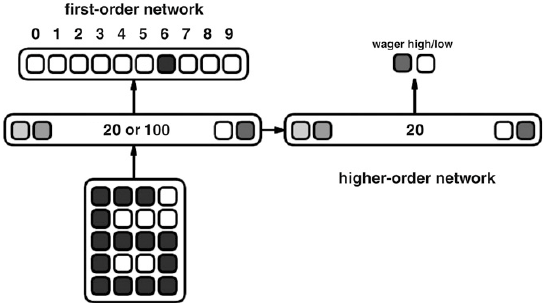
\includegraphics[width=230px]{data/expC1/schema.png}
      \end{center}
      
    \paragraph{Paramètres}
      \begin{center}
	\begin{tabular}{lr}
	  \begin{minipage}{230px}
	    \begin{itemize}
	      \item momentum : 0.5 sur les 2 réseaux
	      \item taux d'apprentissage : 0.15 sur les 2 réseaux
	      \item 10 chiffres différents présentés
	      \item apprentissage 10 (formes) x 300 (époques)
	      \item utilisation de biais
	      \item sigmoïde à température 1
	    \end{itemize}
	  \end{minipage}
	  &
	  \begin{minipage}{230px}
	    \begin{itemize}
	      \item poids initialisés sur [-1 ; 1] pour les 2 réseaux
	      \item taux d'apprentissage constant
	      \item entrées valent 0 ou 1
	    \end{itemize}
	  \end{minipage}
	\end{tabular}
      \end{center}

  
  \newpage
  \subsection{Résultats}
    \paragraph{Principaux}
      Analyse des performances
      \begin{center}
	\begin{tabular}{lr}
	  \hspace*{-1cm}
	  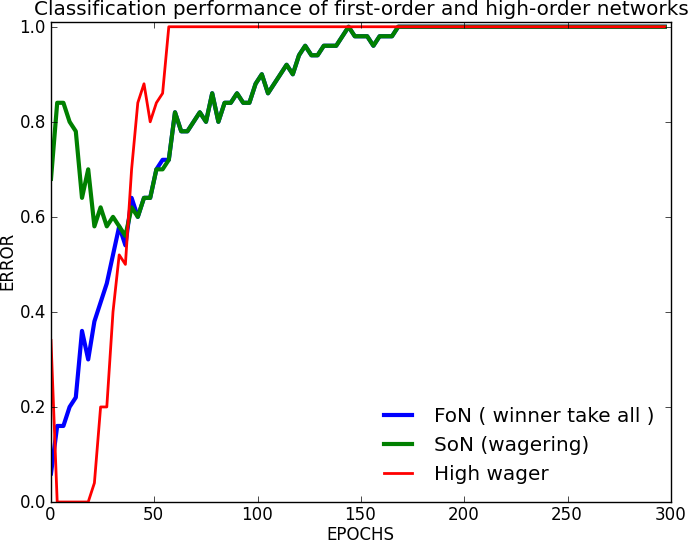
\includegraphics[width=250px]{data/expC1/perf_20.png}
	  &
	  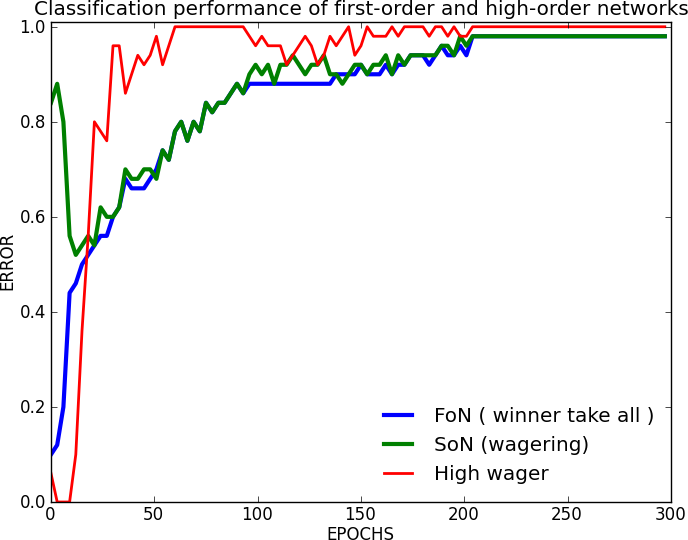
\includegraphics[width=250px]{data/expC1/perf_100.png} \\
	  
	  20 neurones en couche cachée
	  &
	  \hspace*{-1cm}
	  100 neurones en couche cachée
	\end{tabular}
      \end{center}
      \subparagraph{Notes}
	\begin{itemize}
	  \item la courbe rouge représentent le taux de paris hauts du second réseau
	  \item la performance de classification représente le taux de bonnes réponses (winner-take-all) pour les 10 formes présentées sur une époque
	\end{itemize}
      \subparagraph{Conclusion}
	\begin{itemize}
	  \item dans les 2 cas, le premier réseau réussit à apprendre sa tâche de classification
	  \item lorsque le nombre de neurones dans la couche cachée est faible, l'apprentissage de la tâche est optimal, il ne peut plus être amélioré
	  
	  Ainsi le second réseau se contente de parier haut.
	  \item lorsque le nombre de neurones dans la couche cachée est élevé, l'apprentissage peut être amélioré, le second réseau 
	  le remarque et peut accorder son taux de paris hauts avec le taux de succès du premier réseau.
	  
	  Remarquons tout de même qu'avec l'amélioration du second réseau, on ne peut pas dépasser un réseau optimal, seulement l'égaler
	\end{itemize}
    \paragraph{Secondaires}
      RMS
      \begin{center}
	\begin{tabular}{lr}
	  \hspace*{-1cm}
	  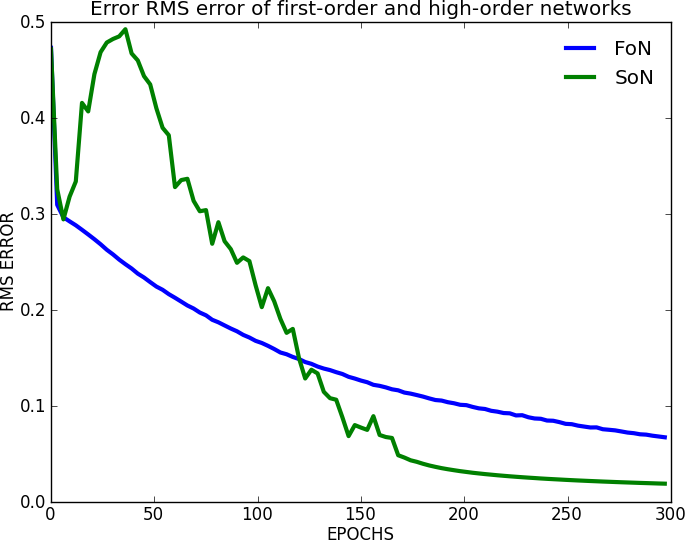
\includegraphics[width=250px]{data/expC1/rms_20.png}
	  &
	  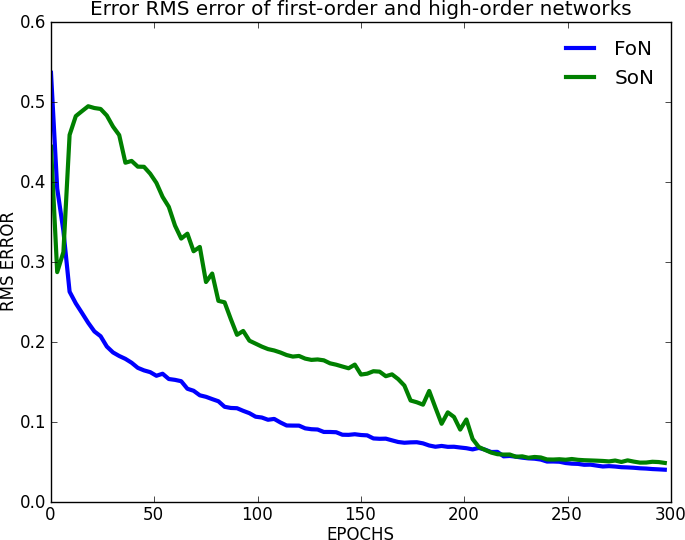
\includegraphics[width=250px]{data/expC1/rms_100.png} \\
	  
	  20 neurones en couche cachée
	  &
	  \hspace*{-1cm}
	  100 neurones en couche cachée
	\end{tabular}
      \end{center} 
      \subparagraph{Notes}
	\begin{itemize}
	  \item formule utilisée pour RMS (cf. Formules~\nameref{rms})
	\end{itemize}
      \subparagraph{Conclusion}
	On remarque que le second réseau apprend et désapprend. De plus, il reste toujours sous la barre
	des 0.5.

  \subsection{Conclusion}
    Comme il l'est dit dans \cite{Cleeremans_2007}, cette architecture tente de résoudre les problèmes des réseaux connexionnistes
  classiques à avoir un semblant de conscience.
  
  À savoir :
  \begin{itemize}
   \item qu'ils ne savent pas qu'ils peuvent se trouver dans différents états, et qu'ils ne traitent pas leurs propres états : 
   d'où la présence de ce second réseau qui tente de traiter ses états et d'apprendre qu'il en a plusieurs
   \item des représentations rentant bloquées dans la chaîne de causalité de la tâche à apprendre : d'où
   le fait que ce second réseau n'affecte pas l'apprentissage du premier (ie. pour ne pas retomber dans la chaîne de causalité)
   \item qu'ils n'ont pas les connaissances conscientes des raisons de leurs décisions : on essaye de les y sensibiliser avec les paris
   \\[0.2cm]
  \end{itemize}
  
  
  Par ailleurs, cette architecture ouvre des possibilités d'amélioration de l'apprentissage.
  Elle permet au réseau de détecter lui même un nombre de neurones trop important dans la couche cachée.
  On pourrait, par exemple, imaginer un réseau autorégulant son nombre de neurone.
  
  L'expérience suivante (\nameref{expC2}) retente l'expérience sur des données réelles.

  \newpage
  \subsection{Formules}
    \paragraph{RMS} \label{rms}
  Pour une époque $e$ :
  \begin{center}
    \begin{large}
    $ rms_{e} = \sqrt{ \frac{1}{n} \sum \limits_{i=1}^{n} 
    ( o_{i,e} - d_{i} )^2 } $
    \end{large}
  $ with \left\lbrace \begin{array}{lll} n : number\ of\ neurons\ on\ the\ output\ 
  layer\\o_{i,e} : value\ obtained\ for\ the\ i^{th}\ neuron\ at\ the\ e^{th}\ epoch\\d_{i} : 
  value\ desired \ for\ the\ i^{th}\ neuron\end{array} \right.$
  \end{center}
    \paragraph{Descente de gradient} \cite{Touzet_1992} \\
  Construction de l'erreur : 
    \begin{center}
      $y_{i} = f'(a_i) \times ( d_i - x_i ) \ si\ i\ neurone\ de\ sortie $ \\
      $y_{i} = f'(a_i) \times \sum \limits_{k} ( w_{ki} \times y_k )\ si\ i\ neurone\ cache $
    \end{center}
  Mise à jour des poids :
    \begin{center}
      $w_{ij}(t+1) = w_{ij}(t) + learning\_rate \times y_{i} \times x_j + momentum \times 
      (w_{ij}(t) - w_{ij}(t-1) )$
    \end{center}
  Variables : 
    \begin{center}
      $\left\lbrace \begin{array}{lll} 
	f : fonction\ sigmoide \\
	x_i : valeur\ du\ neurone\ i\\
	d_i : valeur\ desire pour\ le\ neurone\ i\\
	a_i : somme\ pondere\ des\ poids\ du\ neurone\ i
      \end{array} \right.$
    \end{center}
    
\bibliographystyle{../pre-rapport/apalike}
\bibliography{../pre-rapport/biblio}
